\documentclass[review]{elsarticle}
\usepackage{hyperref}
\usepackage[margin=1in]{geometry}
\usepackage{graphicx}
\usepackage{amsmath}
\usepackage{placeins}
\usepackage{comment}
\usepackage{gensymb}
\usepackage{lineno}


\journal{Journal of Nuclear Materials}
\bibliographystyle{elsarticle-num}

\begin{document}

\begin{frontmatter}
\title{Molecular dynamics investigation of grain boundaries and surfaces in U$_{3}$Si$_{2}$}

\author[inl]{Benjamin Beeler\corref{qwe}}
\cortext[qwe]{Corresponding author}
\ead{benjamin.beeler@inl.gov}
\author[lanl,ucsd,msu]{Michael Baskes}
\author[lanl]{David Andersson}
\author[lanl]{Michael WD Cooper}
\author[inl]{Yongfeng Zhang}
\address[inl]{Idaho National Laboratory, Idaho Falls, ID 83415}
\address[lanl]{Los Alamos National Laboratory, Los Alamos, NM 87545}
\address[ucsd]{University of California-San Diego, San Diego, CA 92093}
\address[msu]{Mississippi State University, MS 39762}

\begin{abstract}

Uranium-silicide (U-Si) fuels are being pursued as a possible accident tolerant fuel (ATF). This uranium alloy benefits from higher thermal conductivity and higher fissile density compared to uranium dioxide (UO$_{2}$). In order to perform engineering scale nuclear fuel performance simulations, the material properties of the fuel must be known. Currently, the experimental data available for U-Si fuels is rather limited. Thus, multi-scale modeling efforts are underway to address this gap in knowledge. Interfaces play a critical role in the microstructural evolution of nuclear fuel under irradiation, acting both as sinks for point defects and as preferential nucleation sites for fission gas bubbles. In this study, a semi-empirical modified Embedded-Atom Method (MEAM) potential is utilized to investigate grain boundaries and free surfaces in U$_{3}$Si$_{2}$. The interfacial energy as a function of temperature is investigated for ten symmetric tilt grain boundaries, eight unique free surfaces and voids of radius up to 35 {\AA}. The point defect segregation energy for both U and Si interstitials and vacancies is also determined for two grain boundary orientations. Finally, the entropy change for grain boundaries is calculated as a function of temperature. This is the first study into grain boundary properties of U-Si nuclear fuel. 

\end{abstract}
\end{frontmatter}

\section{Introduction}

U$_{3}$Si$_{2}$ is being considered as a candidate for accident tolerant fuels (ATFs) for future and existing light-water reactors (LWRs) \cite{zinkle2014, zinkle2016}. ATFs aim to provide additional coping time in the event of an accident (such as a loss of coolant accident) due to the inherent properties of the fuel, while maintaining good operational characteristics. U$_{3}$Si$_{2}$ exhibits higher uranium density than traditional UO$_{2}$ LWR fuel, thus allowing for the possibility of reduced enrichments, fewer assemblies and/or an extended lifetime in the core. U$_{3}$Si$_{2}$ also possesses a higher thermal conductivity than UO$_{2}$, allowing for a lower fuel centerline temperature and more rapid heat removal during off-normal conditions. 

Subjecting U$_{3}$Si$_{2}$ to the in-reactor environment leads to microstructural changes due to the evolution of radiation produced defects, segregation and precipitation of fission products, and mechanical deformation. These changes in fuel microstructure change fuel properties, directly impacting fuel performance and safety. The ability to understand and model microstructural changes throughout the lifetime of the fuel is critical in developing fuel performance modeling codes. In order to perform continuum scale descriptive and predictive nuclear fuel performance simulations, the material properties of the fuel must be known, however, the current experimental data available for U-Si fuels is incomplete. Information that has not yet been investigated via experimentation includes diffusion coefficients, displacement energy, variation of thermal conductivity with porosity, fission product properties within various USi phases and interfacial properties, to name a few. Thus, multi-scale modeling efforts are underway to address this gap in knowledge.

Internal interfaces play a critical role in the determination of mechanical and thermal properties of polycrystalline materials. Specifically in irradiation environments, interfaces act both as sinks for point defects and as preferential nucleation sites for fission gas bubbles. Additionally, interfacial energies are a critical set of properties for the correct implementation of mesoscale modeling. Both the grain boundary and surface energy are utilized within phase-field methods to determine grain growth, void nucleation and bubble evolution. Phase-field models can then incorporate these phenomena to generate swelling predictions for the fuel. Given that fuel swelling is likely a critical aspect governing the operational lifetime of U$_{3}$Si$_{2}$ fuel, incorporation of accurate interfacial properties into phase-field models is an essential step in the multi-scale modeling process.

Because grain boundaries have a significant influence on the physical properties of polycrystalline solids \cite{brandon2010, harmer2010}, their properties, including energy, have been the subjects of extensive experimental and computational study. Interatomic potentials have been successfully employed to study grain boundaries in a variety of systems \cite{morita1997, wolf1989bcc1, wolf1990bcc2, ratanaphan2015, novoselov2014, tschopp2012probing, hahn2016}. This manuscript leverages a recently developed MEAM interatomic potential describing the U-Si system in order to investigate the nature of interfaces in U$_{3}$Si$_{2}$. The interfacial energy as a function of temperature is investigated for ten symmetric tilt grain boundaries, eight unique free surfaces and voids of radius up to 35 {\AA}. The point defect segregation energy for both U and Si interstitials and vacancies is also determined for two grain boundary orientations.. Finally, the entropy and free energy change for a grain boundary is calculated as a function of temperature. This is the first fundamental investigation of the nature, character and energy of interfaces in U$_{3}$Si$_{2}$. 

\section{Computational Details}
Molecular dynamics simulations are performed utilizing the LAMMPS \cite{plimpton1995} software package and the recently published U-Si MEAM potential \cite{beelerUSi}. A supercell with periodic boundaries is generated that contains two grain boundaries or two free surfaces. Ten symmetric tilt grain boundaries are constructed with respect to the [100] tilt axis. Grain boundary system size is dependent upon the interface orientation, ranging from between 600 and 3280 atoms. One unit cell is included in the direction perpendicular to the tilt axis. Eight unique surfaces are investigated, including three different terminations of the [100] direction, a single termination of the (001) direction and a selection of four low symmetry surfaces. The low symmetry surfaces are constructed in the same manner as grain boundaries, however only half of the system is constructed in order to generate two surfaces instead of two grain boundaries. An example system for the U$_{3}$Si$_{2}$ (210) symmetric tilt grain boundary is shown in Fig. \ref{fig:gbex}, where grain boundaries exist in the center of the supercell (denoted by a dashed black line) and on the edges of the periodic supercell.

\begin{figure}[h]
 \centering
 \includegraphics[width=1.0\textwidth]{gbexA.png} 
 \caption{The U$_{3}$Si$_{2}$ (210) symmetric tilt grain boundary at 200 K. Grain boundaries exist in the middle (black dashed line) and on the edges of the supercell. }
 \label{fig:gbex}
\end{figure}

These systems were verified to be large enough to obtain accurate surface energies by investigating a single representative larger system and comparing respective interfacial energies. Relaxation is performed in an NPT-ensemble, relaxing each x, y, and z component individually, with a damping parameter of 0.1. A Langevin thermostat in the Gronbech-Jensen-Farago \cite{gjf2014} formalism is utilized with the damping parameter set to 0.1 ps. Systems are initialized at a temperature of 1600 K, then cooled over 100 ps to the target temperature. The systems are then relaxed for 100 ps, with energies averaged over the final 50 ps. Five unique simulations are performed for each system to ensure statistical significance of the results. The interfacial energy is calculated via equation \ref{eq:surface},

\begin{equation}
\label{eq:surface}
E_{nf}= \frac{(E^{*} - E)}{SA} * N
\end{equation}

where $\it{E^{*}}$ is the energy per atom of the system with two interfaces, $\it{E}$ is the energy per atom of the perfect crystal U$_{3}$Si$_{2}$, $\it{SA}$ is the total surface area of the interface (two interfaces are present in the system) and $\textit{N}$ is the number of atoms in the system with two interfaces. Five unique target temperatures are analyzed - 0 K, 400 K, 800 K, 1200 K and 1600 K - in order to fully investigate the entire regime of phase stability for U$_{3}$Si$_{2}$. 

Voids are constructed by relaxing a 15x15x25 unit cell system consisting of 56,250 atoms for 20 ps at a prescribed temperature, then removing a sphere of atoms from the center of the supercell. The size of the void is progressively increased, starting from a void radius of 5 {\AA} and moving up to a void radius of 35 {\AA}. Equation \ref{eq:surface} is utilized to calculated the void surface energy, where $\it{E^{*}}$ is the energy per atom of the system with a void and SA is the surface area of the void. The stoichiometry of the system is maintained as close to ideal as possible, with an average deviation from ideal stoichiometry of 0.006 {\%}. 

Point defect grain boundary segregation energies are determined by generating a defect (vacancy or interstitial) at a prescribed distance from the grain boundary and analyzing the energy of the system as a function of defect distance from the grain boundary. Two grain boundary orientations were chosen (the (210) and (730) symmetric tilt with respect to the [100] tilt axis), with the simulation setup identical to the calculations on grain boundary energy described above. The defect segregation energy is defined by equation \ref{eq:seg},

\begin{equation}
\label{eq:seg}
E^{seg}(r)= E^{def}(r) - E^{bulk}
\end{equation}

where E$^{def}$ is the energy of the system with a defect at a given distance \textit{r} from the grain boundary and E$^{bulk}$ is defined as the energy of the system with a defect in the bulk (far away from the grain boundary). The bulk is defined as a defect that is 30 {\AA} from the grain boundary, which is sufficiently far from the grain boundary such that no defect-grain boundary interaction is observable. In order to obtain statistical significance of the results, 40 unique simulations were performed for each defect type. Initially, the system is equilibrated at 1600 K for 50 ps, then an atom of a given type, either U or Si, is randomly deleted (vacancy) or inserted (interstitial) from a 3 {\AA} thick slice of the supercell. The system is then equilibrated for another 50 ps to allow the defect to find a reduced energy configuration. The system is then reduced over 50 ps to the target temperature. Finally, the system is equilibrated at the target temperature for 100 ps with the energy of the system averaged over the final 50 ps. The 3 {\AA} slice is then translated along the direction normal (the y-direction in Fig. \ref{fig:gbex}) to the grain boundary in order sample the entire supercell. It should be emphasized that a specific defect configuration is not investigated, only specific defect types. The system is equilibrated at an elevated temperature in order to allow the defect to find a reduced energy configuration. Thus, it is critical to utilize a sufficient sample in order to obtain appropriately averaged defect properties.

The reduction of the free energy of the system determines the manner in which the microstructure of a given system evolves. Thus, in addition to obtaining interfacial energies, it is valuable to investigate the entropy of systems containing grain boundaries as well. The change in entropy of the system is determined by equation \ref{eq:entropy},

\begin{equation}
\label{eq:entropy}
\Delta S = \int_{T_{1}}^{T_{2}} \frac{C_{p}}{T} dT
\end{equation}

where C$_{p}$ is the constant pressure heat capacity in the temperature range T$_{1}$ to T$_{2}$. By integrating, the change in entropy can be evaluated as:

\begin{equation}
\label{eq:entropy2}
\Delta S = C_{p} \times (ln(T_{2}) - ln(T_{1})) 
\end{equation}

The heat capacity is determined by the centered-finite difference approach in equation \ref{eq:cp},

\begin{equation}
\label{eq:cp}
C_{p} = \frac{(TE_{2} - TE_{1})}{(T_{2} - T_{1})} / N
\end{equation}

where TE is the total energy of the system at a given temperature T, and N is the total number of atoms in that system. To ensure that only the grain boundary contribution to the entropy change is being evaluated, the entropy change induced by the bulk is subtracted from the total entropy change of the system with grain boundaries. Additionally, given that grain boundaries are characterized by their specific area, the entropy change of the grain boundary is divided by the grain boundary area, in order to have a normalized system capable of comparing different grain boundary orientations that possess different grain boundary areas within these simulations. 

Finally, the free energy change is determined by equation \ref{eq:free}:

\begin{equation}
\label{eq:free}
\Delta G = \Delta U - T \Delta S
\end{equation}

where $\Delta S$ is taken from equation \ref{eq:entropy} and $\Delta U$ is the change in enthalpy of the system.  Similar to entropy, to ensure that only the grain boundary contribution to the enthalpy change is being evaluated, the enthalpy change induced by the bulk is subtracted from the total enthalpy change of the system with grain boundaries.

\section{Results}
\subsection{Grain boundary energy of U$_{3}$Si$_{2}$}

The U$_{3}$Si$_{2}$ grain boundary energy at 0 K as a function of misorientation angle is shown in Fig. \ref{fig:translate}. Orientations studied within this work are labeled. Data points are connected with straight lines as a means to guide the eye. In Fig. \ref{fig:translate}, both an initial and a post-translation set of data are shown. To ensure that the lowest energy configuration for each grain boundary was obtained, a grain-grain translation was performed prior to relaxation in the direction parallel to the tilt axis. Thus, one grain was held fixed while the other grain was moved. Translation in the x-direction (as denoted in Fig. \ref{fig:gbex}) was performed in increments of 2 {\AA}, sampling the entire grain boundary unit cell. For example, for the (210) grain boundary shown in Fig. \ref{fig:gbex}), the length of the system in the x-direction is approximately 32 {\AA}, thus 16 unique configurations are sampled. In addition, translation is performed for the y- and z-directions. For these directions, a single translation was performed of one half unit cell. The y-direction translation generates a unique surface termination. Thus, four sets of translations are performed: x-direction, x- and y-directions, x- and z-directions, and finally x-, y- and z-directions. This results in a total of 852 unique grain boundary configurations for the 10 symmetric tilt grain boundary orientations. The minimum number of grain boundary configurations for a given misorientation angle is 52. 

The minimum energy configuration found from the translation process is selected as the new configuration for a given misorientation angle. In Fig. \ref{fig:translate}, the initial grain boundary configuration is provided as the blue square data points, while the minimum energy grain boundary found in the translation process is provided as the orange diamond data points. A significant reduction in the grain boundary energy is achievable via grain-grain translation, with an average reduction in the grain boundary energy of approximately 0.3 J/m$^{2}$. The most significant reductions are observed for the (410), (210) and (320) grain boundary orientations. 

\begin{figure}[h]
 \centering
 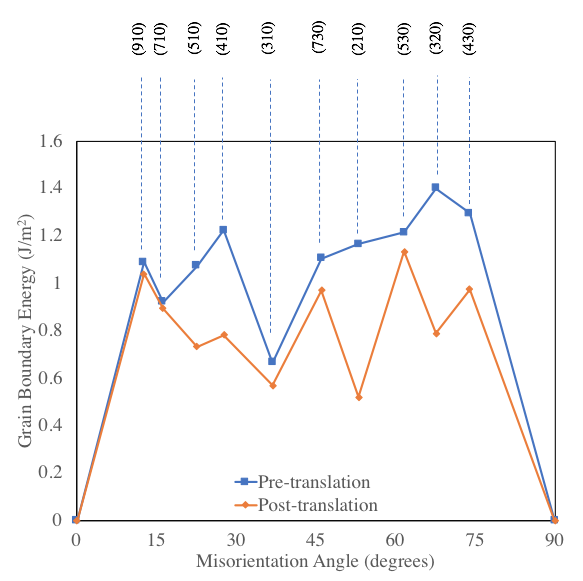
\includegraphics[width=0.6\textwidth]{translation0k.png} 
 \caption{The U$_{3}$Si$_{2}$ grain boundary energy as a function of misorientation angle with respect to the (100) tilt axis at 0 K. Data in blue squares is the initial configuration. Data in orange diamonds is the minimum energy configuration for a given misorientation angle after grain-grain translation.}
 \label{fig:translate}
\end{figure}

\FloatBarrier

Analyzing the post-translation data, the most prominent minima observed are at the (310) and (210) orientations, whereas maxima are observed at the (730) and (530) orientations. The data from Fig. \ref{fig:translate} is displayed in Table \ref{tab:200k}, listing the ten unique symmetric tilt grain boundaries that were investigated for the U$_{3}$Si$_{2}$ system. The average standard deviation for each of these data points is 0.06 J/m$^{2}$. The minimum energy grain boundary orientations examined are the (210) and the (310), while the maximum energy grain boundary orientation examined is the (530), with a difference between the maximum and minimum of 0.57 J/m$^{2}$. 

\begin{table}[h]
\caption{The U$_{3}$Si$_{2}$ grain boundary energy as a function of misorientation angle with respect to the (100) tilt axis at 0 K.} \label{tab:200k}
\begin{center}
\begin{tabular}{|c|c|}
	\hline
	Orientation & Energy (J/m$^{2}$) \\
	 \hline
	 (910) & 0.94 \\
	 (710) & 0.80 \\
	 (510) & 0.78 \\
	 (410) & 0.74 \\
	 (310) & 0.50 \\	 
	 (730) & 0.95 \\
	 (210) & 0.49 \\
	 (530) & 1.06 \\
	 (320) & 0.84 \\
	 (430) & 0.93 \\
	 \hline
\end{tabular}
\end{center}
\label{default}
\end{table}

\FloatBarrier

The grain boundary energy as a function of misorientation angle at five temperatures is displayed in Fig. \ref{fig:gbtemp}. It is observed that the general trend of grain boundary energy as a function of misorientation angle is maintained with increasing temperature. The primary cusps remain at the (210) and (310) orientations and the most prominent maxima remains at the (730) orientation. 

\begin{figure}[h]
 \centering
 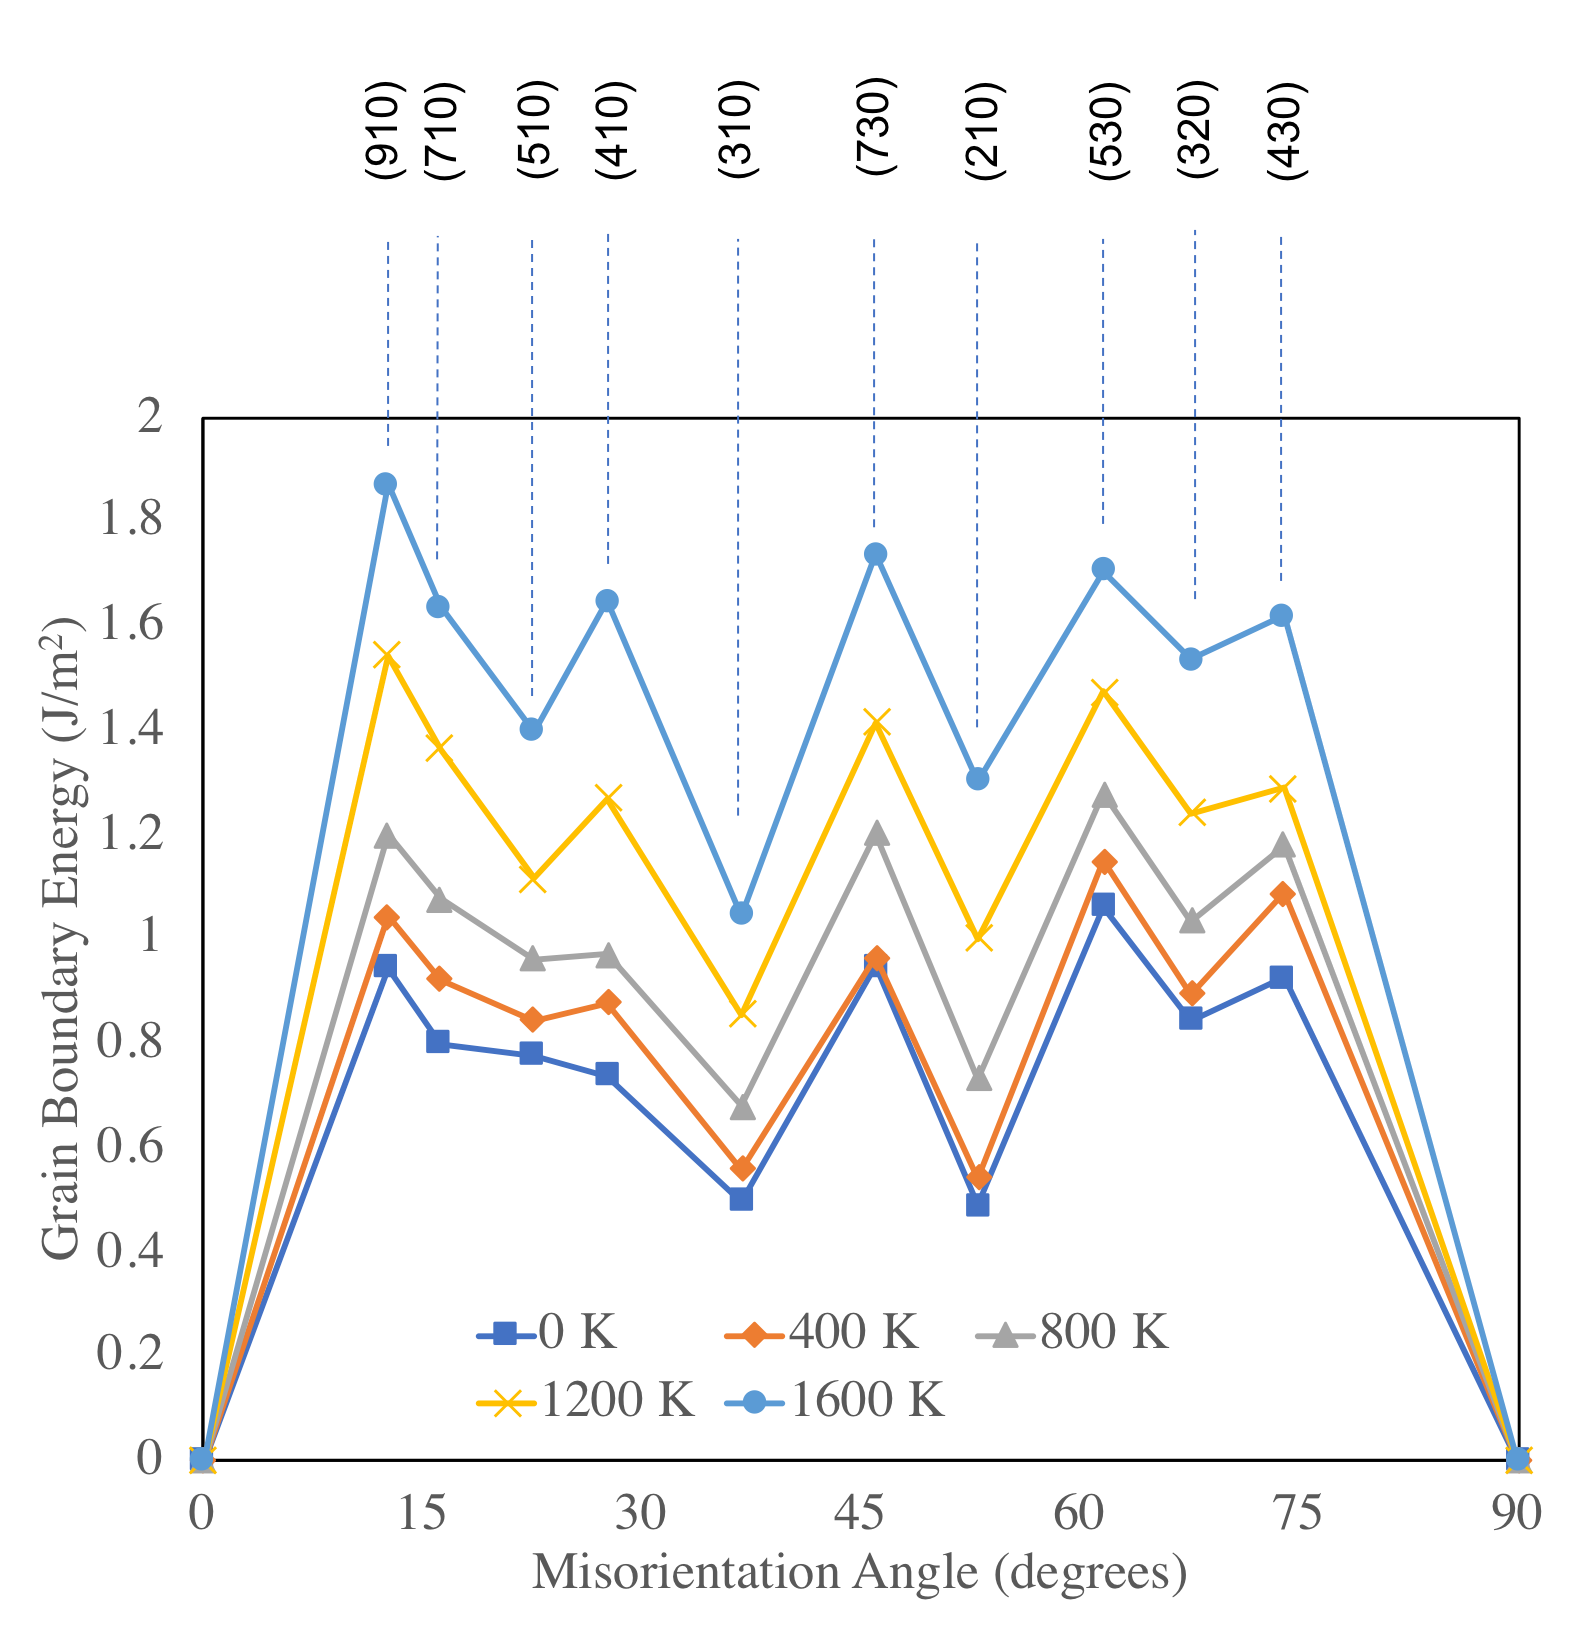
\includegraphics[width=0.8\textwidth]{gb_vs_Ta.png} 
 \caption{The U$_{3}$Si$_{2}$ grain boundary energy as a function of misorientation angle with respect to the (100) tilt axis at 0 K, 400 K, 800 K, 1200 K and 1600 K.}
 \label{fig:gbtemp}
\end{figure}

\FloatBarrier

To discern a more clear dependence of grain boundary energy as a function of temperature, the difference in grain boundary energy with increasing temperature is plotted in Fig. \ref{fig:gbdeltaT} for all ten symmetric tilt grain boundaries. The grain boundary energy for each orientation is compared to a reference state of 0 K (the grain boundary energy at a given temperature minus the grain boundary energy at 0 K for each specific orientation). There is a clear general trend of increasing grain boundary energy with increasing temperature. The average over the data set is also shown in Fig. \ref{fig:gbdeltaT} as a bold black line. The data is most readily fit to a second order polynomial function. There is an average increase in grain boundary energy of 0.05 J/m$^{2}$ per 100 K. The average grain boundary energy at 0 K is 0.80 J/m$^{2}$, at 400 K is 0.89 J/m$^{2}$, at 800 K is 1.03 J/m$^{2}$, at 1200 K is 1.26 J/m$^{2}$ and the average grain boundary energy at 1600 K is 1.55 J/m$^{2}$. The average standard deviation at 1600 K is approximately 0.06 J/m$^{2}$. Thus, this trend of increasing grain boundary energy with increasing temperature is statistically significant.
 
 \begin{figure}[h]
 \centering
 \includegraphics[width=0.8\textwidth]{deltaGB_vs_Ta.png} 
 \caption{The difference in the U$_{3}$Si$_{2}$ grain boundary energy at a given temperature with respect to the grain boundary energy at 0 K for each orientation. The average of the data set is shown as a bold black line. }
 \label{fig:gbdeltaT}
\end{figure}


\FloatBarrier

\subsection{Surface energy of U$_{3}$Si$_{2}$}

The U$_{3}$Si$_{2}$ surface energy for eight unique surfaces is shown in Fig. \ref{fig:surfT}. Three different terminations of the (100) surface are denoted Xa, Xb and Xc, while the (001) termination is denoted as Z. The low symmetry surfaces are denoted by their planar orientation. In Fig. \ref{fig:surfT}, it is observed that the Xc surface has the lowest energy across the entire temperature range investigated, followed by the (310) surface, while the Xb and (210) surfaces are consistently the highest in energy over the temperature range. Visual inspection of free surfaces showed that higher energy surfaces are those that are primarily one species, where one surface is U-rich and the other surface is Si-rich. The lowest energy surfaces are those with a mixed U-Si character. The relative magnitudes of the surface energies for each orientation generally maintain the same sequence with increasing temperature. The data from Fig.\ref{fig:surfT} is displayed in Table \ref{tab:surfT}.

\begin{figure}[h]
 \centering
 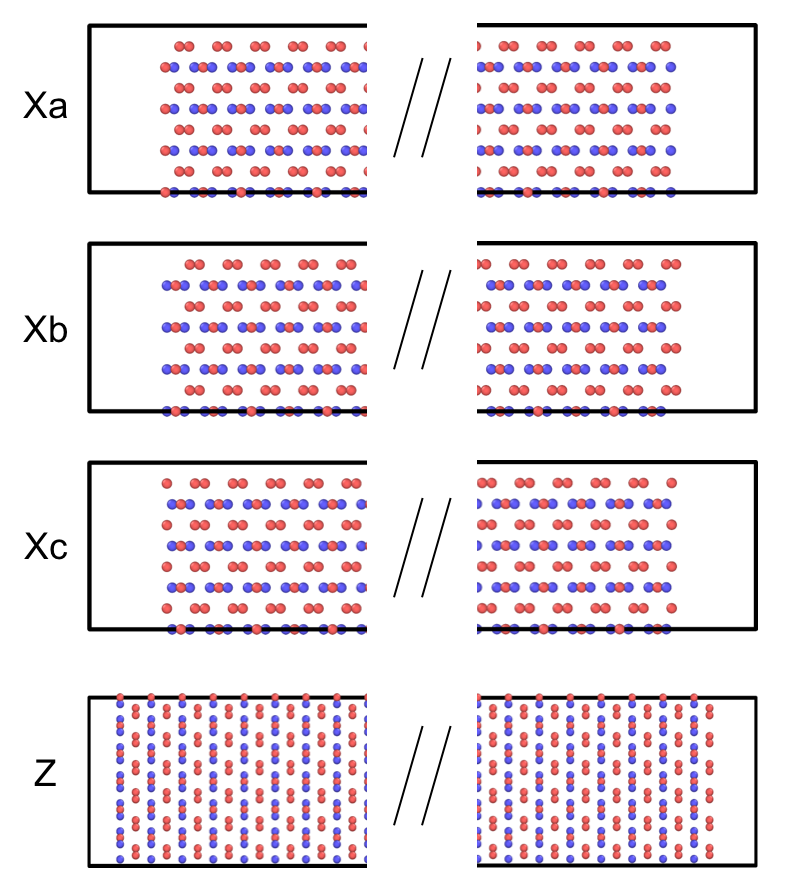
\includegraphics[width=0.6\textwidth]{surfX.png} 
 \caption{The unique U$_{3}$Si$_{2}$ surface terminations in the X- and Z- directions. }
 \label{fig:surfT}
\end{figure}

\begin{figure}[h]
 \centering
 \includegraphics[width=0.8\textwidth]{surf_vs_Ta.png} 
 \caption{The U$_{3}$Si$_{2}$ surface energy as a function of temperature for eight unique surface terminations. }
 \label{fig:surfT}
\end{figure}

\begin{table}[h]
\caption{The U$_{3}$Si$_{2}$ surface energy as a function of temperature for eight unique surface terminations. Units in J/m$^{2}$.} \label{tab:surfT}
\begin{center}
\begin{tabular}{|c|c|c|c|c|c|}
	\hline
	Orientation & 0 K & 400 K & 800 K & 1200 K & 1600 K\\
	 \hline
	 Xa & 1.74	 & 1.71 & 1.72 & 1.76 & 1.90 \\
	 Xb & 1.87 & 1.85 & 1.80 & 1.81 & 1.94 \\
	 Xc & 1.59	 & 1.59 & 1.58 & 1.67 & 1.92 \\
	 Z & 1.74 & 1.74 & 1.75 & 1.79 & 1.93 \\
	 (210) & 1.83 & 	1.79 & 1.77 & 1.83 & 2.04 \\
	 (310) & 1.63 & 1.64 & 1.66 & 1.74 & 2.00 \\	 
	 (410) & 1.70 & 1.71 & 1.74 & 1.81 & 1.97 \\
	 (510) & 1.68 & 1.68 & 1.69 & 1.76 & 1.95 \\
	 \hline
\end{tabular}
\end{center}
\label{default}
\end{table}

\FloatBarrier

To more clearly ascertain the influence of temperature on surface energy, the difference in surface energy with increasing temperature is plotted in Fig. \ref{fig:deltasurf} for all eight surface orientations. The surface energy for each orientation is compared to a reference state of 0 K. This data is averaged, shown as a bold black line in Fig. \ref{fig:deltasurf}. There is negligible variation in the average surface energy with increasing temperature up to 800 K. At 1200 K, there is a slight increase in average surface energy, followed by a substantial increase at 1600 K. The average surface energy as a function of temperature is given in Table \ref{tab:surf}. 

\begin{figure}[h]
 \centering
 \includegraphics[width=0.8\textwidth]{deltasurfvsTa.png} 
 \caption{The difference in the U$_{3}$Si$_{2}$ surface energy at a given temperature with respect to the surface energy at 0 K for each orientation. The average over all eight orientations is shown as a bold black line. }
 \label{fig:deltasurf}
\end{figure}

\begin{table}[h]
\caption{The U$_{3}$Si$_{2}$ average surface energy as a function of temperature.} \label{tab:surf}
\begin{center}
\begin{tabular}{|c|c|c|c|c|c|}
	\hline
	Temperature (K) & Surface energy (J/m$^{2}$)\\
	 \hline
	 0 & 1.72	  \\
	 400 & 1.71  \\
	 800 & 1.71	  \\
	 1200 & 1.77  \\
	 1600 & 1.95  \\
	 \hline
\end{tabular}
\end{center}
\label{default}
\end{table}

\FloatBarrier

\subsection{Void surface energy of U$_{3}$Si$_{2}$}

One methodology for determining an average surface energy is to investigate the surface energy of a void. The surface energy of a void was calculated as a function of radius and temperature, with the results shown in Fig. \ref{fig:void}. For all temperatures, the void surface energy converges above a void radius of approximately 20 {\AA}, whereafter an increase in the radius does not change the magnitude of the surface energy. At void sizes above 20 {\AA} in radius, there is no statistically significant difference in the void surface energy as a function of temperature for systems at 0 K, 400 K and 800 K. These three temperatures converge to a void surface energy of approximately 1.74 J/m$^{2}$. The converged void surface energy across all temperatures is presented in Table \ref{tab:void}. The value for void surface energy is within the range of values observed for free surfaces in section 3.2, and as such these two results can be viewed as self-consistent. Above 800 K, the void surface energy increases slightly at 1200 K, then increases substantially at 1600 K. This is also consistent with the findings from free surface simulations in section 3.2. 




\begin{figure}[h]
 \centering
 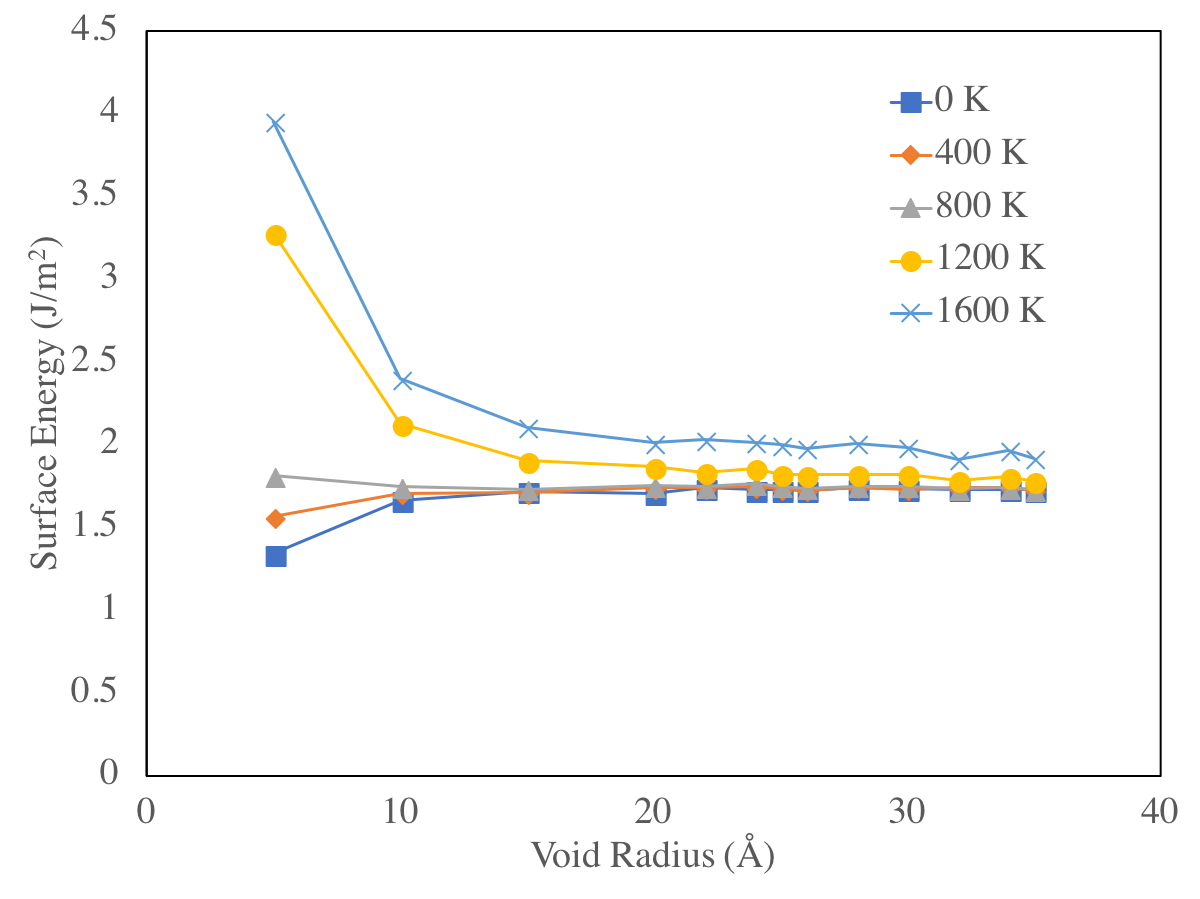
\includegraphics[width=0.8\textwidth]{void_vs_rb.png} 
 \caption{The U$_{3}$Si$_{2}$ void surface energy as a function of radius at five distinct temperatures. }
 \label{fig:void}
\end{figure}

\begin{table}[h]
\caption{The U$_{3}$Si$_{2}$ void surface energy as a function of temperature.} \label{tab:void}
\begin{center}
\begin{tabular}{|c|c|c|c|c|c|}
	\hline
	Temperature (K) & Surface energy (J/m$^{2}$)\\
	 \hline
	 0 & 1.73	  \\
	 400 & 1.74  \\
	 800 & 1.74	  \\
	 1200 & 1.80  \\
	 1600 & 1.95  \\
	 \hline
\end{tabular}
\end{center}
\label{default}
\end{table}

Visual inspection of large voids was conducted to determine the nature of the difference in void surface energy at very high temperatures. As would be expected, at higher temperatures there exists a greater degree of surface roughening and surface reorientation. The thermal motion of the system near the melting point (previously calculated as approximately 1775 K \cite{beelerUSi}) leads to bond breaking and local deviation from crystallinity, resulting in higher surface energies. This also explains the variability in free surface energy with increasing temperature shown in Table \ref{tab:surf}. Additional variance is observed in the small void regime (r $<$ 20 {\AA}), where a higher temperature yields a higher void surface energy. This can be explained from a two-fold effect: 1) bond breaking from very high temperatures increasing the energy of the system, and 2) smaller voids have smaller surface area and thus less ability to reorganize and reduce the energy of the system. 

\FloatBarrier

\subsection{Point defect grain boundary segregation energies}

The defect segregation energy for four defect types at a (730) symmetric tilt grain boundary as a function of distance from the grain boundary is shown in Fig. \ref{fig:defects730} at 0 K, 400 K, 800 K, and 1200 K. The four defect types are the U vacancy, U interstitial, Si vacancy and Si interstitial. Although there are two unique uranium sites in the U$_{3}$Si$_{2}$ crystal structure, an averaged U vacancy defect formation energy is utilized in this work, as outlined in the computational details. It can be observed that for each defect type investigated, there is a general attraction near the grain boundary, which manifests as a negative segregation energy per equation \ref{eq:seg}. This affinity for defects to reside in or near grain boundaries is very short range for all defects analyzed, in that beyond approximately 10 {\AA} there is no statistically significant attraction. There is some noticeable scatter in the data points, even for defects residing far away from the grain boundary. This is due to different possible defect sites and thermal fluctuations in the simulations. However, a large enough sample set of data is generated to have statistical confidence in the results.

\begin{figure}[h]
 \centering
 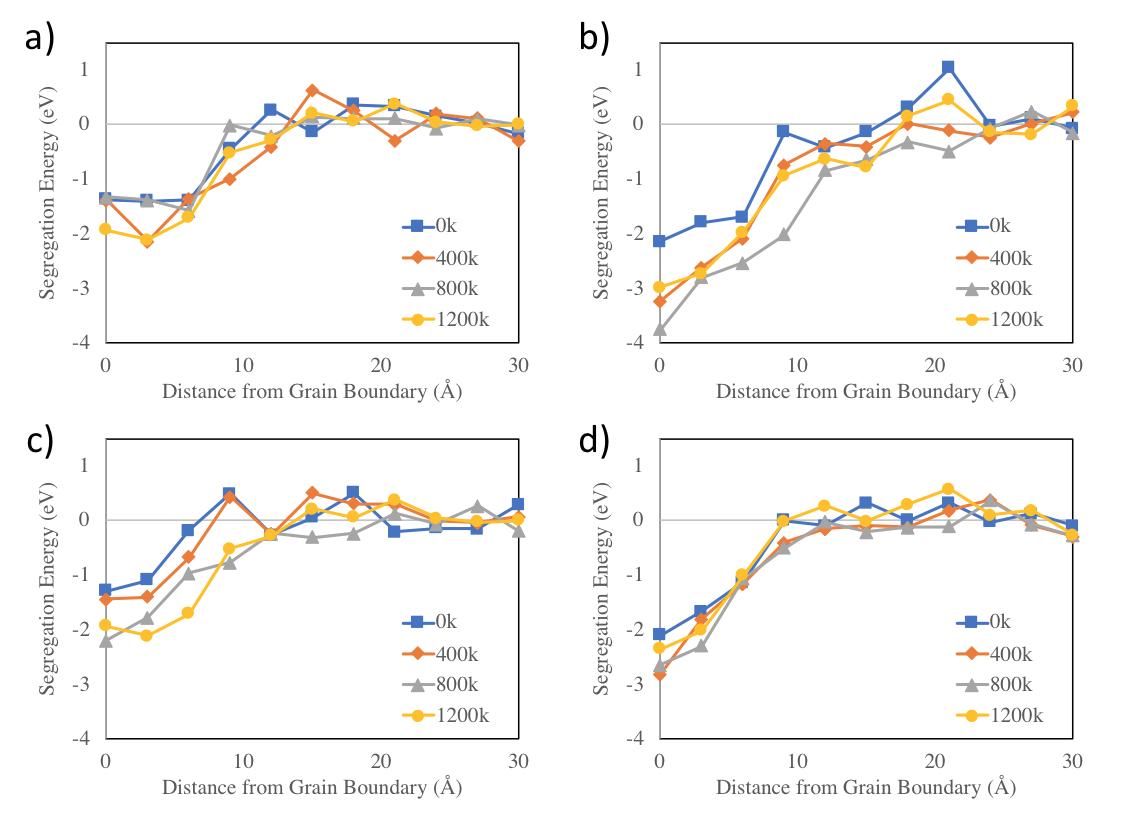
\includegraphics[width=0.8\textwidth]{defectsB730.png} 
 \caption{Point defect segregation energy as a function of distance from the grain boundary. Each defect is investigated at four different temperatures. Defects shown are a) U vacancy, b) U interstitial, c) Si vacancy and d) Si interstitial. }
 \label{fig:defects730}
\end{figure}

\begin{comment}

\begin{figure}[h]
 \centering
 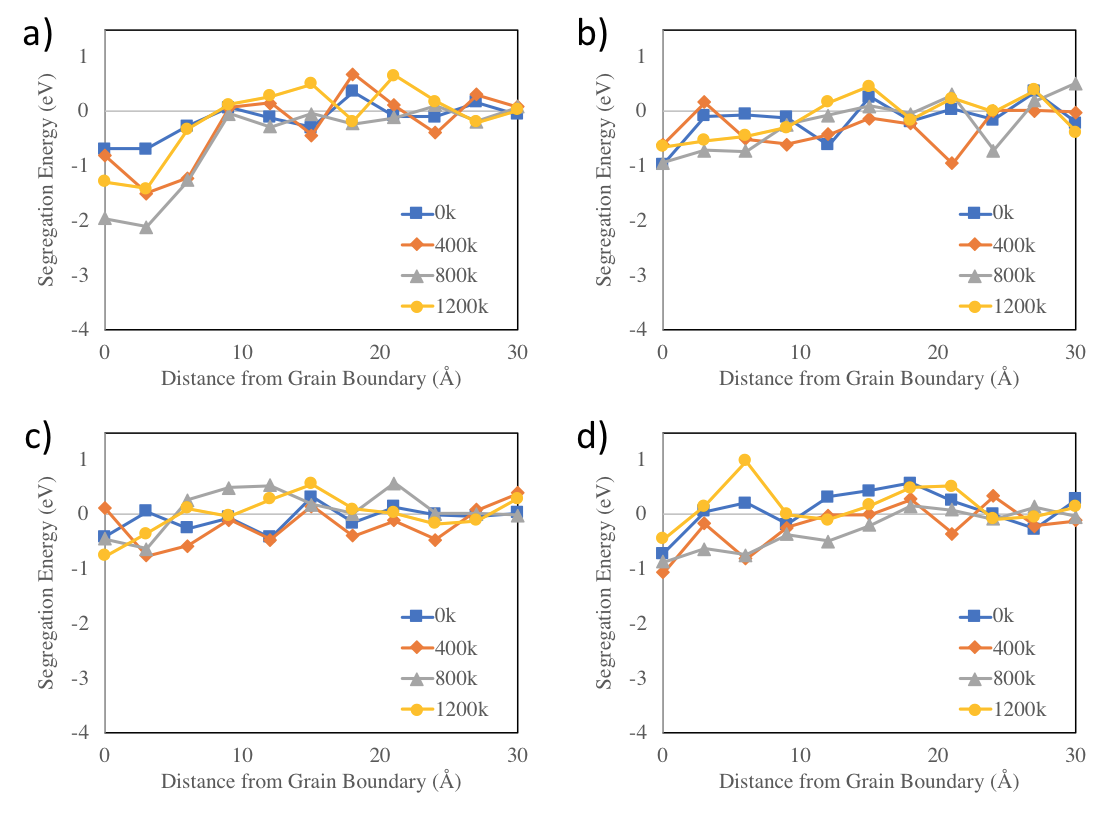
\includegraphics[width=0.8\textwidth]{defectsB210.png} 
 \caption{Point defect segregation energy as a function of distance from the grain boundary. Each defect is investigated at four different temperatures. Defects shown are U vacancy, U interstitial, Si vacancy and Si interstitial. }
 \label{fig:defects210}
\end{figure}

\end{comment}

Averaging over the entire data set for each defect type, the general behavior for a given defect can be more readily determined, and more easily compared to other defect types and other grain boundary orientations. The average of the data set for each defect type is plotted in Fig. \ref{fig:seg}. Additionally, the same set of simulations is performed for a (210) symmetric tilt grain boundary. The average of the data set for the (210) grain boundary is also shown in Fig. \ref{fig:seg}. It can be observed that all defect types exhibit a more negative segregation energy for the (730) symmetric tilt grain boundary compared to the (210) symmetric tilt grain boundary. Referring back to the grain boundary energies from section 3.1, the grain boundary energy for the (730) orientation is much higher than that of the (210) orientation. Thus, the higher energy grain boundary exhibits a stronger preference to attract and absorb point defects.

\begin{figure}[h]
 \centering
 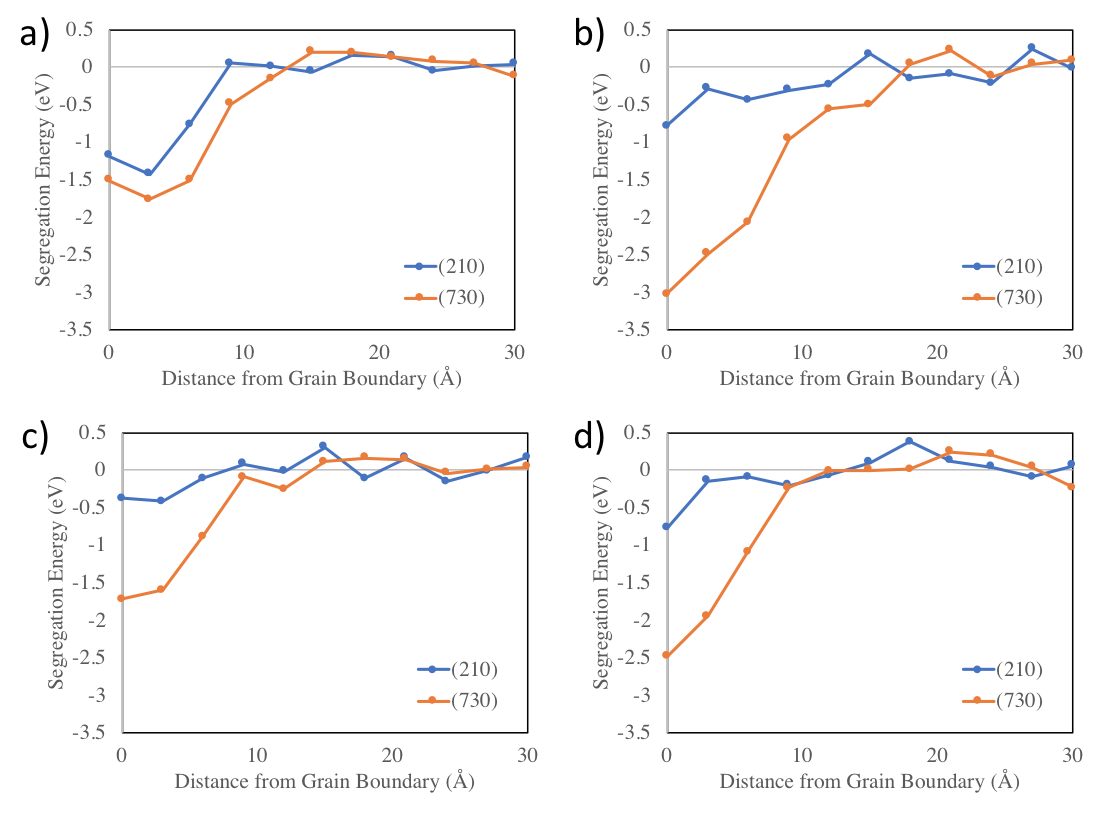
\includegraphics[width=0.8\textwidth]{defects_avg.png} 
 \caption{Average point defect segregation energy as a function of distance from the grain boundary for four defect types and two grain boundary orientations. Defects shown are a) U vacancy, b) U interstitial, c) Si vacancy and d) Si interstitial.  }
 \label{fig:seg}
\end{figure}

\FloatBarrier

There is no clear trend on which defects are most attracted to grain boundaries, as the relative magnitudes of segregation energies for point defects changes depending on the grain boundary orientation. For the (730) grain boundary, interstitials of both U and Si display the strongest attraction, while for the (210) grain boundary, U vacancies display the strongest attraction. A summary of segregation energies (averaged over the 0 {\AA} and 3 {\AA} data points) is shown in Table \ref{tab:seg}. 

\begin{table}[h]
\caption{The U$_{3}$Si$_{2}$ average point defect segregation energy. Units in eV.} \label{tab:seg}
\begin{center}
\begin{tabular}{|c|c|c|c|c|c|}
	\hline
	Defect Type & (730) & (210)\\
	 \hline
	 U vac & -1.64 & -1.31	  \\
	 U int & -2.76 & -0.54 \\
	 Si vac & -1.66 & -0.40	  \\
	 Si int & -2.21 & -0.46 \\
	 \hline
\end{tabular}
\end{center}
\label{default}
\end{table}

This study on point defects was extended to systems at 1600 K. However, the temperature was sufficiently high, and the segregation energy sufficiently large, that defects near the grain boundaries diffused into the grain boundaries. Thus, the systems did not allow for the calculation of a segregation energy as a function of distance from the grain boundary. However, these simulations did provide additional verification that defects will preferentially reside near or in the grain boundary. 

\FloatBarrier

\subsection{Grain boundary thermodynamics}

Utilizing the variation of total energy with temperature from simulations in section 3.1, the constant-pressure heat capacity (C$_{p}$), entropy change and free energy change can be calculated via equations \ref{eq:entropy}~-~\ref{eq:free}. The calculation of heat capacity is based on the central finite difference of total energy over temperature. In Fig. \ref{fig:entropy}, the change in entropy for ten symmetric tilt grain boundary orientations is shown relative to 400 K, with an average overlaid as a bold black line. The entropy change increases with increasing temperature. The average total entropy change from 400 K to 1600 K is approximately 3.3x10$^{-3}$ J/mol-K-{\AA}$^{2}$. It should be noted that the entropy change is given on a per area basis. The bulk entropy change over this temperature range is 35 J/mol-K, which is similar in magnitude to previous studies determining entropy changes in carbon nanocrystals \cite{mcnutt2014}. The change in entropy is lowest for the (910) and (710) low angle grain boundaries, which is qualitatively coherent.

\begin{figure}[h]
 \centering
 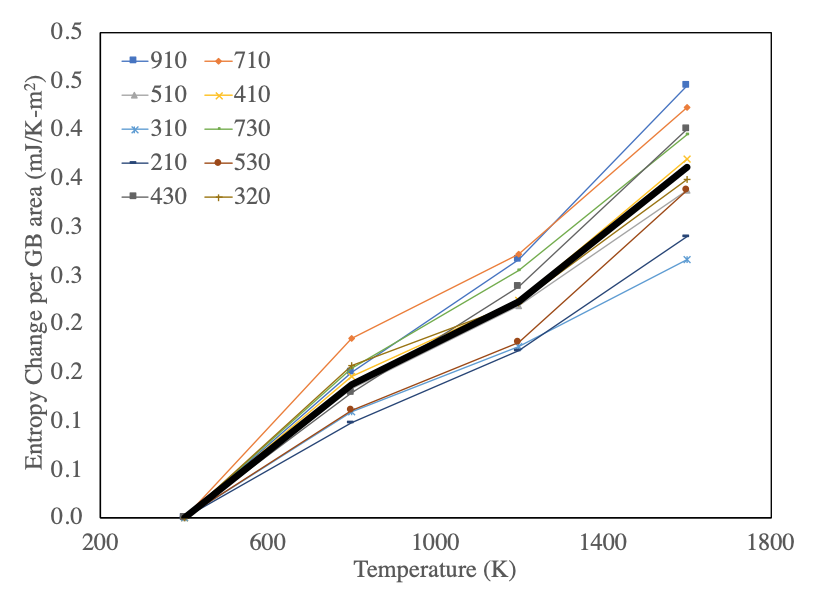
\includegraphics[width=0.6\textwidth]{entropy.png} 
 \caption{Change in entropy as a function of temperature for ten symmetric tilt grain boundaries.}
 \label{fig:entropy}
\end{figure}

The change in free energy as a function of temperature is shown In Fig. \ref{fig:free} for ten symmetric tilt grain boundary orientations relative to 400 K. An average is overlaid as a bold black line. The free energy change decreases with increasing temperature, resulting in lower free energies at higher temperatures due to the increasing entropy of the system. This is qualitatively consistent with previous work on thermodynamic integration of grain boundaries in Cu \cite{frolov2012} and Ni \cite{foiles2010}. 

\begin{figure}[h]
 \centering
 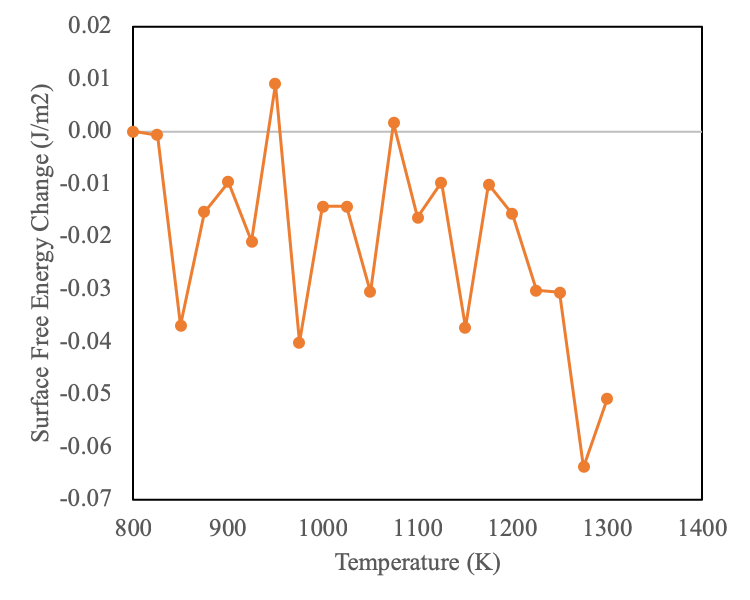
\includegraphics[width=0.6\textwidth]{free.png} 
 \caption{Change in free energy as a function of temperature for ten symmetric tilt grain boundaries.}
 \label{fig:free}
\end{figure}

\FloatBarrier

\section{Conclusions}

In this study a recently developed MEAM interatomic potential was utilized to investigate the nature of interfaces in U$_{3}$Si$_{2}$. This was the first fundamental investigation of the nature, character and energy of interfaces in U$_{3}$Si$_{2}$. The interfacial energy as a function of temperature was investigated for ten symmetric tilt grain boundaries. The (210) and (310) grain boundary orientations exhibited the lowest grain boundary energy and the average grain boundary energy for U$_{3}$Si$_{2}$ increased from 0.80 J/m$^{2}$ at 0 K to 1.55 J/m$^{2}$ at 1600 K. Eight unique free surfaces were investigated, with the finding that the Xc and (310) surfaces are the lowest in energy over the temperature range of interest. The free surfaces in U$_{3}$Si${_2}$ exhibit a trend towards increasing surface energy with increasing temperature above 1200 K. Voids in U$_{3}$Si$_{2}$ of radius up to 35 {\AA} were also investigated. The void surface energy converges to a value of 1.74 J/m$^{2}$ once a void reaches a radius of 20 {\AA}. The void surface energy displays similar variance with increasing temperature as that observed in free surfaces. The point defect segregation energy was also determined for two grain boundary orientations, showing that U and Si vacancies and interstitials display a preference to reside near the grain boundary. This energetic preference diminishes once the defect is more than 10 {\AA} from the grain boundary. Additionally, the segregation energy was greater in magnitude for the higher energy grain boundary. Finally, the entropy and free energy change for grain boundaries was calculated as a function of temperature. The entropy change increases with increasing temperature, leading to a decrease in the free energy with increasing temperature. 

The information within this manuscript can be utilized by mesoscale methodologies to study a variety of phenomena. The inclusion of realistic grain boundary, surface energies and free energy changes allows for the investigation of grain growth, void formation, void morphology and swelling in U$_{3}$Si$_{2}$. Realistic segregation energies can be incorporated to parametrize sink strengths utilized in phase-field defect evolution models. The ability to accurately describe each of these phenomena is critical in understanding microstructural evolution of nuclear fuel in-reactor. 

\section{Acknowledgement}
This work is supported by the U.S. Department of Energy, Office of Nuclear Energy, Nuclear Energy Advanced Modeling and Simulation (NEAMS) Program. This work is also supported by U.S. Department of Energy, Office of Nuclear Energy, Nuclear Energy University Partnerships, under contract no. DE-NE0008564. This manuscript has been authored by Battelle Energy Alliance, LLC under Contract No. DEAC07-05ID14517 with the U.S. Department of Energy. The United States Government retains and the publisher, by accepting the article for publication, acknowledges that the United States Government retains a nonexclusive, paid-up, irrevocable, world-wide license to publish or reproduce the published form of this manuscript, or allow others to do so, for United States Government purposes.  Los Alamos National Laboratory, an affirmative action/equal opportunity employer, is operated by Los Alamos National Security, LLC, for the National Nuclear Security Administration of the U.S. Department of Energy under Contract No. DE-AC52-06NA25396.  This research made use of the resources of the High Performance Computing Center at Idaho National Laboratory, which is supported by the Office of Nuclear Energy of the U.S. Department of Energy and the Nuclear Science User Facilities under Contract No. DE-AC07-05ID14517.

\section{References}

\bibliography{MARMOTbib}


\end{document} 
